
\section{funzioni trigonometriche, radianti}
%%%%%%%%%%%
%%%%%%%%%%%

Nel capitolo~\ref{sec:avvolgimento} abbiamo definito le 
funzioni $\sin$ e $\cos\colon \RR\to \RR$ con periodo $\tau>0$ (arbitrario)
in modo tale che la funzione $\phi\colon \RR\to\RR^2$, $\phi(t)=(\cos t, \sin t)$ 
percorra, con moto circolare uniforme, in senso antiorario, la circonferenza 
unitaria $\ENCLOSE{(x,y)\in \RR^2\colon x^2+y^2=1}$.
Tale funzione descrive in effetti un moto circolare uniforme 
in quanto percorre archi congruenti in tempi uguali.
\mynote{Due figure geometriche sono \emph{congruenti} se c'è una isometria 
che manda una nell'altra.
Due archi sono congruenti se hanno la stessa lunghezza e lo stesso raggio, 
ma non è necessario introdurre il concetto di \emph{lunghezza d'arco} per parlare 
di congruenza.
}

Vogliamo ora mostrare che è possibile scegliere la costante $\tau$
in modo tale che la linea descritta da $\phi$ percorra la circonferenza 
con \emph{velocità} unitaria.
\mynote{Ricordiamo che $\tau$ è il periodo delle funzioni $\phi$,
$\cos$ e $\sin$}%
Se seguo il punto $f(t)$ a partire dall'istante $t=0$ per un breve tempo 
$\Delta t\neq 0$
osservo che il punto si sposta tra $f(0) = (1,0)$ e 
$f(\Delta t) = (\cos \Delta t, \sin \Delta t)$.
\mynote{La notazione $\Delta t$ indica un qualunque numero positivo.
Usiamo tale notazione perché tale numero rappresenta 
una differenza ($\Delta$ è una lettera $D$ greca)
di tempi tra loro vicini.}%
Intuitivamente quando $t=0$ il punto $f(t)$ si muove verticalmente, 
verso l'alto. 
Lo spazio percorso $\Delta s$ sarà quindi approssimativamente 
uguale alla variazione della coordinata $y$: 
$\Delta y = \sin \Delta t$.
\mynote{Ricordiamo che $\sin 0 = 0$}
Dunque la velocità sarà pari alla componente verticale della velocità 
e sarà, intuitivamente, il limite di $\frac{\Delta y}{\Delta t}$ ovvero 
\mynote{Vedremo tra poco che questo limite è la  
\emph{derivata} della funzione $f$ nel punto $t=0$.}
\[
\lim_{\Delta t\to 0} \frac{\sin(\Delta t)}{\Delta t}.  
\]

Dal punto di vista formale non è del tutto ovvio che questo limite esista.
Nel seguito lo dimostriamo, con un metodo molto simile a quello utilizzato 
per definire la costante $e$ di Nepero.
Così come l'esponenziale reale $x\mapsto a^x$ 
è un isomorfismo tra il gruppo additivo di $\RR$ e il gruppo moltiplicativo 
di $\RR^+$, così la funzione $\phi(t) = (\cos(t), \sin(t))$ 
risulta essere un isomorfismo 
tra il gruppo additivo $\RR$ e il gruppo delle rotazioni del piano che può essere 
rappresentato dall'insieme $U$ dei numeri complessi unitari.
Abbiamo già visto che affinché il punto che si muove con legge 
oraria $x\mapsto a^x$ abbia velocità $1$ per $x=0$ 
si deve porre $a=e$, la base dei logaritmi naturali.
Allo stesso modo vedremo ora che affinché la velocità 
del punto $t\mapsto \phi(t)$ 
sia anch'essa unitaria bisogna avere $\tau = 2\pi$.
Mettendo assieme i due isomorfismi $e^t$ e $\phi(t)$ si potrà definire,
come vedremo tra poco, un isomorfismo tra il gruppo additivo $\CC$ 
e il gruppo moltiplicativo $\CC\setminus\ENCLOSE 0$.
Quello che si ottiene è l'esponenziale complesso $z\mapsto e^z$. 
La velocità di $\phi(t)$ rappresenta in effetti la derivata di tale funzione 
complessa nel punto $1$ nella direzione dell'asse immaginario 
così come la derivata della funzione esponenziale reale è la derivata 
nella direzione reale. 
Si intuisce così come le costanti fondamentali $e$ e $\pi$ siano legate 
tra loro dalla condizione di fare sì che la funzione esponenziale complessa 
sia derivabile in senso complesso ed abbia derivata complessa pari a $1$.

\subsection{il numero $\pi$}

In questo capitolo dobbiamo lavorare con le funzioni 
$\sin$, $\cos$ e $\tg=\frac{\sin }{\cos}$ introdotte 
nel capitolo~\ref{sec:avvolgimento}. 
Queste funzioni sono state definite con un periodo $\tau>0$
fissato in modo arbitrario. 
Scriveremo 
$\sin_\tau$ 
e $\cos_\tau$ invece di $\sin$ e $\cos$ se è utile mettere in evidenza 
la dipendenza da $\tau$.

\begin{theorem}[limite notevole $\sin$]
Per ogni $\tau>0$, $x\in \RR$, $x\neq 0$, la successione
\[
    a_n = \frac{\sin_\tau \frac xn} {\frac xn}
\]
converge ad un limite positivo (e finito).
\end{theorem}
%
\begin{proof}
Faremo uso della funzione $\tg x= \frac{\sin x}{\cos x}$.
Useremo le formule di addizione:
\begin{align*}
 \sin(x+y) &= \sin x\cos y + \cos x \sin y,\\
 \cos(x+y) &= \cos x \cos y - \sin x \sin y  
\end{align*}
da cui, facendo il rapporto e dividendo numeratore 
e denominatore per $\cos x \cos y$ si ottiene:
\[
  \tg(x+y) = \frac{\tg x + \tg y}{1-\tg x \tg y}.
\]
Useremo anche il fatto che sull'intervallo 
$\closeinterval{0}{\frac \tau 4}$
\mynote{ricordiamo che $\tau$ è il periodo (scelto arbitrariamente)
delle funzioni $\sin$ e $\cos$} 
la funzione $\sin$ è crescente, la funzione $\cos $
è decrescente ed entrambe hanno valori compresi 
tra $0$ e $1$.
Tutte queste proprietà sono garantite 
dal teorema~\ref{th:proprieta_trigonometriche}.

\emph{Passo 1:}
vogliamo dimostrare che se $n$ è un intero positivo 
e $x>0$ è tale che $0\le nx <\frac \tau 4$ allora si ha
\begin{equation}\label{eq:4813509}
  \sin n x \le n\sin x\le \tg nx.
\end{equation}
Possiamo dimostrare per induzione l'implicazione 
$nx\le \frac \tau 4 \implies$~\eqref{eq:4813509}.
Se $n=1$ è ovvio.
Supponiamo allora che \eqref{eq:4813509} 
sia valida per un certo $n$ e che  
sia $(n+1)x<\frac \tau 4$. 
Allora da un lato si ha
\begin{align*}
  \sin (n+1)x 
  &= \sin nx \cdot \cos x + \cos nx\sin x
  \le \sin nx + \sin x
\end{align*}
e usando l'ipotesi induttiva $\sin nx\le n\sin x$ 
si ottiene 
\[
 \sin(n+1)x \le n\sin x+\sin x = (n+1)\sin x  
\]
che è la prima disuguaglianza che dovevamo dimostrare.
Per l'altra disuguaglianza osserviamo che si ha 
\begin{align*}
  \tg(n+1)x 
  &= \frac{\tg nx + \tg x}{1-\tg nx \tg x}
  \ge \tg nx + \tg x
  \ge \tg nx + \sin x
\end{align*}
e applicando l'ipotesi induttiva 
$\tg nx\ge n\sin x$ si ottiene 
\[
 \tg(n+1)x 
 \ge n\sin x +\sin x 
 =   (n+1)\sin x
\]
come volevamo dimostrare.

\emph{Passo 2:}
dimostriamo che se $x>0$,
posto
\[
  a_n = \frac{\sin \frac x n}{\frac x n} = \frac{n\sin \frac x n}{x}
\]
si ha $a_{n+1}\ge a_n$ per ogni $n \ge \frac{4x}{\tau}$
e dunque, essendo definitivamente monotona, 
la successione ammette limite 
(grazie al teorema~\ref{th:limite_monotona}):
$a_n \to \ell$ per $n\to +\infty$.
Posto $y=\frac{x}{n(n+1)}$ basta mostrare che 
se $\frac{x}{n} \le \frac{\tau}{4}$, si ha
\[
  (n+1) \sin ny \ge n \sin (n+1)y.  
\]
Ma usando $n\sin y\le \tg ny$ da~\eqref{eq:4813509} si ha 
\begin{align*}
  n \sin(n+1)y
  &=n(\sin ny\cos y + \cos ny \sin y) \\
  &\le n\sin ny + n\sin y\cos ny\\
  &\le n\sin ny + \tg ny\cos ny\\
  &= (n+1)\sin ny
\end{align*}
che è quanto volevamo dimostrare.

\emph{Passo 3.}
vogliamo mostrare che il limite $\ell=\lim a_n$ è positivo e 
finito.
Basta osservare che se $x>0$ e $\frac x m <\frac \tau 4$
per $m$ intero sufficientemente grande, 
usando~\eqref{eq:4813509} con 
con $\frac x {mn}$ al posto di $x$,
si ha $\sin \frac x m \le n\sin\frac x {m n} \le \tg \frac{x}{m}$ 
e quindi
\[
  \frac{\sin \frac x m}{\frac x m} 
  \le \frac{\sin \frac x {mn}}{\frac x {mn}} 
  \le \frac{\tg \frac x m}{\frac x m}.
  \]
Sappiamo che la sottosuccessione $a_{mn}\to \ell$ e, dunque,
dovrà essere 
\[
  0 <
  \frac{\sin \frac x m}{\frac x m} 
  \le \ell
  \le \frac{\tg \frac x m}{\frac x m} < +\infty.
\]

\emph{Conclusione.}
Abbiamo dimostrato il teorema per ogni $x>0$.
Se $x<0$ il risultato si ottiene per simmetria usando: 
$\sin(-x)=-\sin x$.
\end{proof}

Se applichiamo il teorema precedente 
con $\tau=1$ e $x=1$ otteniamo che la successione 
$a_n = n\cdot \sin_1\enclose{\frac 1 n}$ converge 
ad una costante universale.
In particolare avendo posto la misura dell'angolo giro pari a 
$\tau=1$, l'angolo di misura $\frac 1 n$ 
è l'angolo formato dal lato di un $n$-agono 
regolare inscritto nella circonferenza unitaria.
Dunque $a_n$ non è altro che il perimetro di tale 
$n$-agono regolare e il limite a cui tende deve essere,
geometricamente, la lunghezza della circonferenza unitaria.

Questo dà significato geometrico alla seguente definizione.

\begin{definition}[$\pi$ costante fondamentale della trigonometria]%
  \label{def:pi}%
Definiamo
\[
 \pi 
  \defeq \frac 1 2 \lim_{n\to +\infty} n\cdot \sin_1 \enclose{\frac 1 n}.
\]
dove $\sin_1$ è la funzione $\sin$ costruita nel 
teorema~\ref{def:sin_cos} con periodo $\tau=1$.
\end{definition}

\begin{theorem}[limite notevole $\sin$]
  \label{th:limite_notevole_sin}%
Sia $\sin_\tau$ la funzione seno definita 
dal teorema~\ref{def:sin_cos} con periodo $\tau>0$.
Per ogni $x\in\RR$, $x\neq 0$ si ha 
\[
\lim_{x\to 0}\frac{\sin_{\tau} x}{x}
= \frac{2\pi}{\tau}.
\]
\end{theorem}
%
\begin{proof}
Risulta ovviamente $\sin_\tau(\tau x) = \sin_1 x$ in quanto 
la funzione $\sin_\tau(\tau x)$ ha periodo $1$ e soddisfa tutte le proprietà 
enunciate nel teorema~\ref{def:sin_cos}.
Ora per ogni $x>0$ esiste $n\in \NN$ tale che 
$\frac \tau {n+1} \le x \le \frac \tau n$ 
e se $nx<\frac \tau 4$ usando la monotonia della funzione $\sin_\tau$ 
si ottiene:
\begin{align*}
  n \sin_1 \frac 1 {n+1}
  = n \sin_\tau \frac \tau {(n+1)}
  \le n \sin_\tau x 
  = n \sin_1 \frac x \tau 
  \le n \sin_1 \frac 1 n.
\end{align*}
Ovviamente se $x\to 0^+$ si ha $n=n(x)\to +\infty$.
Per come abbiamo definito $\pi$ 
sappiamo che $n \sin_1 \frac 1 n\to 2\pi$ per $n\to +\infty$
e visto che $n\sim n+1$ entrambi i lati della precedente equazione 
tendono allo stesso limite $2\pi$ e dunque, per confronto, 
\[
  \lim_{x\to 0^+} \tau \cdot \frac{\sin_\tau x}{x} = 2\pi.  
\]
Per simmetria lo stesso limite vale quanto $x\to 0^-$
e si ottiene dunque il risultato voluto.
\end{proof}

D'ora in avanti sceglieremo $\tau=2\pi$ come periodo 
delle funzioni trigonometriche.
E d'ora in avanti si intenderà $\sin = \sin_{2\pi}$, 
$\cos = \cos_{2\pi}$. Si avrà quindi il limite notevole 
\[
   \lim_{x\to 0} \frac{\sin x}{x} = 1.  
\]

Quando introdurremo le derivate potremo anche osservare che 
questa scelta del periodo $\tau=2\pi$ 
fa sì che il punto di coordinate
$(\cos t,\sin t)$ si muova con velocità unitaria lungo 
la circonferenza unitaria. 
Dunque tale punto percorre un arco di lunghezza $t$ nel tempo $t$.
In particolare in un periodo $\tau=2\pi$ il punto percorre l'intera 
circonferenza e dunque risulta che $2\pi$ è la lunghezza 
della circonferenza unitaria (ovvero $2\pi r$ è la lunghezza della circonferenza 
di raggio $r$).
Al tempo $t=1$ il punto $(\cos t,\sin t)$ individua un angolo che 
viene chiamato \emph{radiante} in quanto corrisponde ad un arco di lunghezza 
pari al raggio (unitario). 
Dunque il \emph{radiante} è l'unità di misura naturale per misurare gli angoli 
e le funzioni $\sin$ e $\cos$ d'ora in poi saranno fissate con tale unità di misura.

\newsavebox{\qrfigtrigo}\sbox{\qrfigtrigo}{\myurlhere{figtrigo}{funzioni trigonometriche}}%
\begin{figure}
  \centering%
  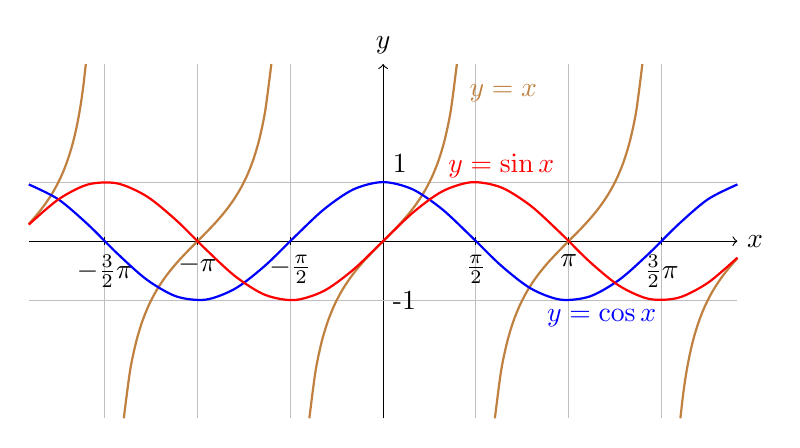
\begin{tikzpicture}[scale=0.75]
  \draw[->] (-6,0) -- (6,0) node[right] {$x$};
  \draw[->] (0,-3) -- (0,3) node[above] {$y$};
  \foreach \x/\xtext in
    {{pi/2}/{\frac \pi 2}, {pi}/{\pi}, {3*pi/2}/{\frac{3}{2}\pi},
    {-pi/2}/{-\frac \pi 2}, {-pi}/{-\pi}, {-3*pi/2}/{-\frac{3}{2}\pi}} {
    \draw[shift={(\x,0)},lightgray] (0,-3) -- (0,3);
    \draw[shift={(\x,0)}] (0pt,2pt) -- (0pt,-2pt) node[below] {$\xtext$};
  }
  \foreach \y in {1, -1} {
    \draw[shift={(0,\y)},lightgray] (-6,0) -- (6,0);
  }
  \draw (0,1) node [above right] {1};
  \draw (0,-1) node [right] {-1};
  \draw[domain=-rad(atan(3)):rad(atan(3)),smooth,variable=\x,brown,thick] plot ({\x},{tan(deg(\x))});
  \draw[domain=pi-rad(atan(3)):pi+rad(atan(3)),smooth,variable=\x,brown,thick] plot ({\x},{tan(deg(\x))});
  \draw[domain=-pi-rad(atan(3)):-pi+rad(atan(3)),smooth,variable=\x,brown,thick] plot ({\x},{tan(deg(\x))});
  \draw[domain=-6:-2*pi+rad(atan(3)),smooth,variable=\x,brown,thick] plot ({\x},{tan(deg(\x))});
  \draw[domain=2*pi-rad(atan(3)):6,smooth,variable=\x,brown,thick] plot ({\x},{tan(deg(\x))});
  \draw[domain=-6:6,smooth,variable=\x,blue,thick] plot ({\x},{cos(deg(\x))});
  \draw[domain=-6:6,smooth,variable=\x,red,thick] plot ({\x},{sin(deg(\x))});
  \draw (3.7,-1) node[blue,below] {$y=\cos x$};
  \draw (2,0.9)  node[red,above] {$y=\sin x$};
  \draw (1.3,2.5) node[brown,right] {$y=\tg x$};
  \end{tikzpicture}
  \caption{%
  I grafici delle funzioni $\sin$, $\cos$ e $\tg$.
  \ifwidemargin\\\\\fi%
  \usebox{\qrfigtrigo}}
\end{figure}

\subsection{funzioni trigonometriche inverse}

La funzione $\sin\colon[-\pi/2,\pi/2]\to [-1,1]$ 
risulta essere strettamente crescente e bigettiva. 
Dunque restringendo il dominio all'intervallo $[-\pi/2, \pi/2]$
e il codominio all'intervallo $[-1,1]$ la funzione risulta invertibile.
La funzione inversa
\[
  \arcsin\colon[-1,1]\to [-\pi/2, \pi/2]
\]
si chiama \emph{arco seno}. 
Per definizione di funzione inversa si ha
\[
  \arcsin(\sin x) = x, \qquad \forall x \in [-\pi/2, \pi/2]
\]
e
\[
  \sin(\arcsin x) = x, \qquad \forall x \in [-1, 1].
\]

La funzione $\cos \colon[0,\pi] \to [-1,1]$ risulta essere strettamente
decrescente e bigettiva.
La funzione inversa
\[
  \arccos\colon[-1,1] \to [0,\pi]
\]
si chiama \emph{arco coseno}. Per definizione si ha
\[
  \arccos(\cos x) = x, \qquad \forall x \in [0,\pi]
\]
e
\[
    \cos(\arccos x) = x, \qquad \forall x \in [-1,1].
\]

La funzione
\index{tangente!funzione trigonometrica}
\mymargin{$\tg x$}%
\index{$\tg x$}
\[
\tg x = \frac{\sin x}{\cos x}
\]
è definita quando $\cos x\neq 0$ ovvero:
\[
  \tg \colon \RR \setminus\ENCLOSE{\frac \pi 2+ k\pi\colon k\in \ZZ} \to \RR.
\]
Se restringiamo la funzione all'intervallo $\enclose{-\pi/2, \pi/2}$ possiamo
facilmente osservare che la funzione $\tg\colon(-\pi/2,\pi/2)\to \RR$ è strettamente crescente. Inoltre se $a_n \to \pi/2$, $a_n<\pi/2$ si ha $\cos(a_n)\to 0$ (per continuità del coseno) e $\sin(a_n)\to 1$ dunque $\tg a_n\to +\infty$. Analogamente per $a_n \to -\pi/2$ si trova $\tg a_n \to -\infty$. Dunque per il teorema dei valori intermedi possiamo affermare che la funzione $\tg\colon(-\pi/2,\pi/2)\to \RR$ è suriettiva. E' quindi invertibile
e la funzione inversa
\[
  \arctg \colon \RR \to (-\pi/2,\pi/2)
\]
si chiama \emph{arco tangente}. Per definizione si ha
\[
  \arctg \tg x = x, \qquad \forall x \in (-\pi/2, \pi/2)
\]
e
\[
  \tg\arctg x = x, \qquad \forall x \in \RR.
\]

Grazie al teorema~\ref{th:monotona_continua}
visto che queste funzioni sono monotone e bigettive
possiamo affermare che
le funzioni $\arcsin$, $\arccos$ e $\arctg$ 
sono tutte funzioni continue.

\begin{exercise}[funzioni misteriose]
  Si disegni il grafico delle seguenti funzioni
  \[
    f(x) = \arcsin \sin x, \qquad 
    g(x) = \arccos \cos x, \qquad 
    h(x) = \arctg \tg x.
  \]
  Si osservi che:
  \begin{enumerate} 
    \item $f$ e $g$ sono definite su tutto $\RR$,
  mentre $h$ è definita su $\RR\setminus\ENCLOSE{\frac{\pi}2+k\pi\colon k\in \ZZ}$;
    \item $f$ e $h$ hanno valori 
  in $\closeinterval{-\frac \pi 2}{\frac \pi 2}$
  mentre $g$ ha valori in $\closeinterval{0}{\pi}$;
    \item $f$ e $g$ hanno periodo $2\pi$,
  $h$ ha periodo $\pi$;
    \item tutte e tre sono funzioni continue (sul loro dominio).
  \end{enumerate}
\end{exercise}

\begin{exercise}
Dimostrare che per ogni $x>0$ si ha
\[
  \arctg \frac 1 x = \frac \pi 2 - \arctg x.
\]
\end{exercise}

\begin{exercise}[lunghezza della circonferenza]
Si osservi che un $n$-agono regolare iscritto a una circonferenza 
di raggio $r$ ha lati di lunghezza $l_n = 2r\sin \frac{\pi}{n}$
e quindi perimetro $p_n = n\cdot l_n$.
Si verifichi che 
\[
  \lim_{n\to +\infty} p_n = 2\pi r.
\]
\end{exercise}
